% Le titre de la partie
\section{Conclusion}

%%%%%%%%%%%%%%%%%%%%%%%%%%%%%%%%%%%%%%%%%%%%%%%%
% Première diapo avec un exemple de tableau
%%%%%%%%%%%%%%%%%%%%%%%%%%%%%%%%%%%%%%%%%%%%%%%%
\begin{frame}
\frametitle{Conclusion}
\framesubtitle{Modèles mathématiques : Sectorisation de la ville}
\begin{figure}
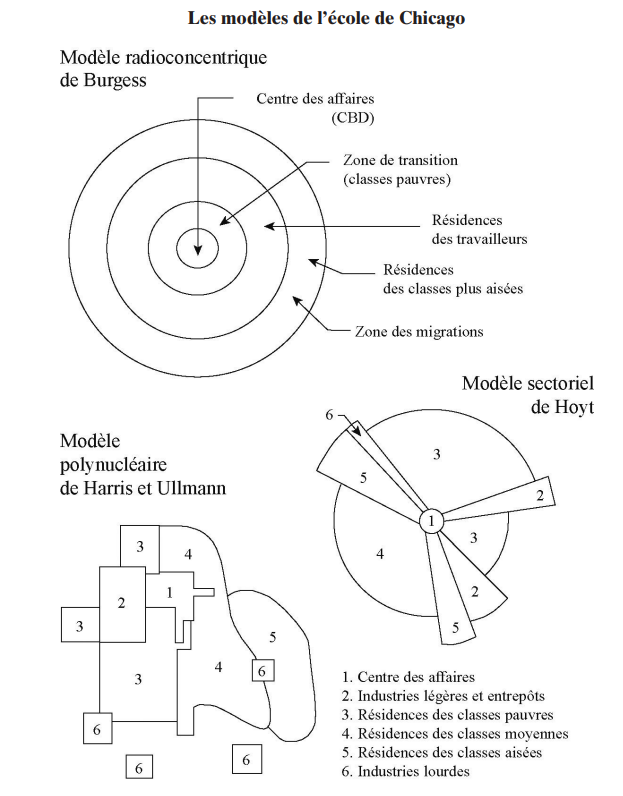
\includegraphics[scale=.27]{diapo/Fig04.png}
\caption{Différentes modélisations de la ville - Formes urbaines et politiques de transport. Jean-Philippe Antoni. Economica,
2011}
\end{figure}


\end{frame}



\begin{frame}
    \frametitle{Questions}
    \framesubtitle{Compléments et ressources}
    
\begin{center}
        
\includegraphics[scale=.4]{diapo/Fig02.png}
    \end{center}
\end{frame}


\begin{frame}
    \frametitle{Questions}
    \framesubtitle{Compléments et ressources}
    
\begin{center}
        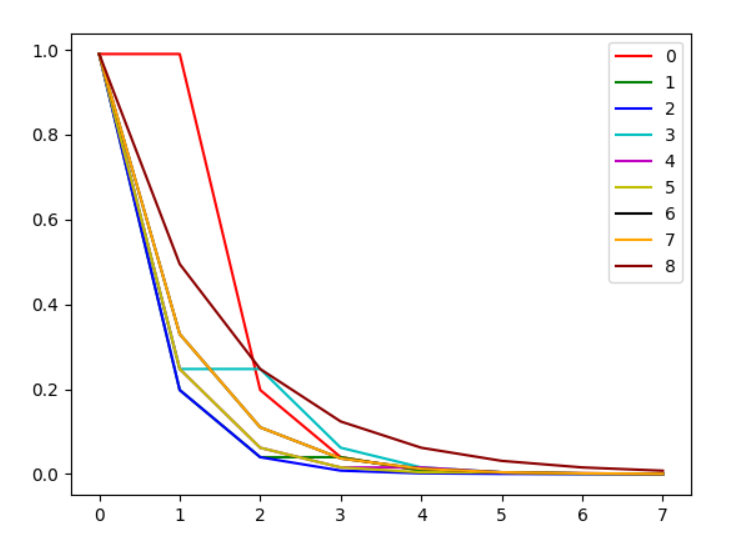
\includegraphics[scale=.3]{diapo/figures/besoins.png}
    \end{center}
\end{frame}
